\chapter{Bayes Factors in the Courtroom}
\label{ch:bf}

\section{From simple to composite hypotheses}

When both propositions specify the probability of the evidence completely, the Bayes factor is the likelihood ratio of Chapter~\ref{ch:odds}. Most legal propositions are not like that. The prosecution says the defendant is the source of a stain, but the probability of the observed profile under that proposition depends on laboratory error rates, on degradation and on the possibility of a mixture. The defence says some unknown person is the source, but the probability of the profile depends on the population that person comes from and on how related he might be to the defendant. In employment discrimination, the claimant says the employer's hiring rate for a protected group was lower than for others; the employer says any difference is chance. Each proposition is composite, a family of distributions indexed by unknown parameters.\index{Bayes factor!composite hypotheses}

The Bayes factor for composite hypotheses averages the likelihood over the parameters under each hypothesis, using a prior distribution for the parameters:
\begin{equation}
\BF_{pd} = \frac{\int \Prob(E\given \theta, \Hp)\,\pi(\theta\given\Hp)\,d\theta}{\int \Prob(E\given \phi,\Hd)\,\pi(\phi\given\Hd)\,d\phi} = \frac{m_p(E)}{m_d(E)} .
\label{eq:bfcomposite}
\end{equation}
The numerator and denominator are marginal likelihoods, the probability of the evidence predicted by each account once its internal uncertainty has been integrated out. The Bayes factor is the ratio of predictive success \citep{kass1995}. It still multiplies prior odds to give posterior odds, so all of the reasoning of Chapter~\ref{ch:odds} carries over. What changes is that the expert must now be explicit about the parameters and their priors, and about how sensitive the result is to them.

\section{DNA profiles with error}

Consider a single source DNA profile. Let $\gamma$ be the random match probability in the relevant population, and let $\epsilon$ be the probability that the laboratory reports a match when the defendant's profile differs from that of the trace, through contamination, sample mixing or interpretive error. Then under $\Hp$ the probability of a reported match is close to one, and under $\Hd$ it is approximately $\gamma + \epsilon$. The Bayes factor is
\begin{equation}
\BF \approx \frac{1}{\gamma + \epsilon}.
\label{eq:dnaerror}
\end{equation}
If $\gamma = 10^{-9}$ and $\epsilon = 10^{-3}$, the Bayes factor is about one thousand, not one billion. The error rate swamps the match probability. Jonathan Koehler and others have argued for decades that juries should be told laboratory error rates for exactly this reason, and that reporting astronomically small match probabilities without them misleads \citep{koehler1993,thompson2003}. The National Research Council's second report on DNA evidence took a different view, preferring to deal with error through retesting rather than by folding an error rate into the statistic \citep{nrc1996}. The Bayesian analysis shows why the issue cannot be avoided: whatever the procedure, the probability of the evidence under the defence hypothesis includes every way in which an innocent person could be reported as matching.\index{DNA evidence!laboratory error}

\section{Low template DNA and transfer}

Modern profiling can produce results from a few cells. With such low template samples, alleles may drop out, spurious alleles may drop in, and DNA may arrive by secondary transfer, carried by a handshake or a shared towel, rather than by direct contact with the crime. The probabilistic genotyping software now used in many jurisdictions computes Bayes factors from models of drop out, drop in and peak heights. These models answer the question of whose DNA is present. They do not answer how or when it got there, which is often the real issue.

A simple model makes the point. Let $c$ be the probability that DNA of the defendant would be found on the item through an innocent route such as transfer or contamination, and let $d$ be the probability of drop out of the defendant's profile if he did touch the item. Under $\Hp$ the probability of detecting the profile is $1-d$. Under $\Hd$ it is $c + (1-c)\gamma$ (a simplification, since drop out is not applied to a coincidental match). The Bayes factor is
\begin{equation}
\BF = \frac{1-d}{c + (1-c)\gamma}.
\label{eq:lowtemplate}
\end{equation}
Figure~\ref{fig:lowtemplate} plots \eqref{eq:lowtemplate}. When the innocent transfer probability is one in a hundred, the Bayes factor cannot exceed one hundred, however rare the profile. This is the central issue in the Kercher case taken up in Chapter~\ref{ch:stories}, where the significance of a trace on a knife and a bra clasp turned on contamination rather than on the rarity of the profile.\index{low template DNA}

\begin{figure}[t]
\centering
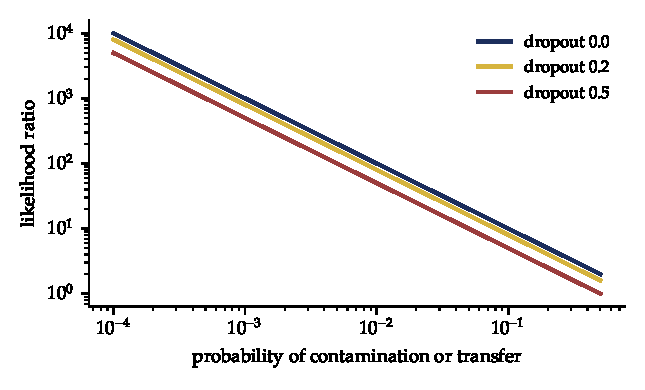
\includegraphics[width=\linewidth]{fig_lowtemplate}
\caption{Bayes factor for a low template DNA detection as a function of the probability of innocent transfer or contamination, for a profile with random match probability $10^{-9}$, at three drop out rates.}
\label{fig:lowtemplate}
\end{figure}

\section{The database search controversy}

Chapter~\ref{ch:classic} worked the search version of the island problem. When a suspect is found by searching a database of profiles, rather than by investigation, does the search weaken the evidence? The second National Research Council report recommended multiplying the match probability by $n$, the number of profiles in the database, on the analogy of a multiple comparisons correction \citep{nrc1996}. Balding and Donnelly argued the opposite, that a database search slightly strengthens the case against the matching individual, because it eliminates the other people in the database as possible sources \citep{balding2005}.\index{database search}

The Bayesian analysis clarifies the question, provided one is careful about the hypothesis. If the question is whether the matching individual is the source, the relevant likelihood ratio is still about $1/\gamma$, and the search has excluded $n-1$ people from the pool of alternatives, so the posterior odds rise slightly. If the question is whether the database contains the source at all, the probability of finding at least one match by chance is about $n\gamma$, and the frequentist correction answers that question. The two camps were answering different questions. What matters is the prior: a person found by trawling a database usually has no other evidence against him, so the prior is the uniform $1/N$ of the island problem of Chapter~\ref{ch:odds}, with $N$ the number of people who could be the source, the defendant included, while a person found by investigation may have a much higher prior. The danger in cold hit cases is not that the likelihood ratio is wrong but that the prior is low and the rest of the case is thin.

\section{Bayes factors and p values}

Statistical evidence in discrimination cases, in antitrust, and in many regulatory disputes is often presented through significance tests. In \emph{Castaneda v Partida} and \emph{Hazelwood School District v United States}, both decided by the United States Supreme Court in 1977, the Court suggested that a disparity of more than two or three standard deviations between the observed and expected numbers of a group would raise suspicion of discrimination \citep{castaneda1977,hazelwood1977}. Lower courts have since often treated a p value below five per cent as a threshold. Chapter~\ref{ch:fienberg} discusses \emph{Castaneda} in detail.\index{p value}\index{Castaneda v Partida}

A p value is not a Bayes factor and not a probability that the null hypothesis is true. For a point null hypothesis tested against a range of alternatives, the Bayes factor implied by a given p value depends on the sample size and on the prior for the alternative. Sellke, Bayarri and Berger showed that, under broad conditions, the Bayes factor in favour of the alternative cannot exceed
\begin{equation}
\overline{\BF}(p) = \frac{-1}{e\, p\log p}, \qquad p < 1/e,
\label{eq:sbb}
\end{equation}
with $\log$ the natural logarithm, which for $p = 0.05$ is about $2.5$ and for $p = 0.01$ is about $8$ \citep{sellke2001}. A result that just reaches conventional significance therefore provides at most modest evidence against the null, rarely enough by itself to meet even a civil standard unless the prior odds are close to even. Conversely, a small p value in a large sample can be paired with weak or even contrary Bayes factors, which is the phenomenon Lindley identified.\index{Sellke Bayarri Berger bound}

\section{Lindley's paradox}

Lindley's paradox concerns a point null hypothesis $H_0 : \theta = 0$ tested against $H_1 : \theta \sim N(0,\tau^2)$, with data summarised by a sample mean whose standard error is $1/\sqrt{n}$. Suppose the observed $z$ statistic is fixed at two, just significant at the five per cent level. The Bayes factor in favour of the null is
\begin{equation}
\BF_{01} = \sqrt{1 + n\tau^2}\,\exp\left(-\frac{z^2}{2}\frac{n\tau^2}{1+n\tau^2}\right),
\label{eq:lindleybf}
\end{equation}
which grows without bound as $n$ increases \citep{lindley1957}. A result that is significant at five per cent in a large sample becomes strong evidence for the null against a diffuse alternative as $n$ grows. Figure~\ref{fig:lindley} shows the Bayes factor as $n$ grows.\index{Lindley's paradox}

\begin{figure}[t]
\centering
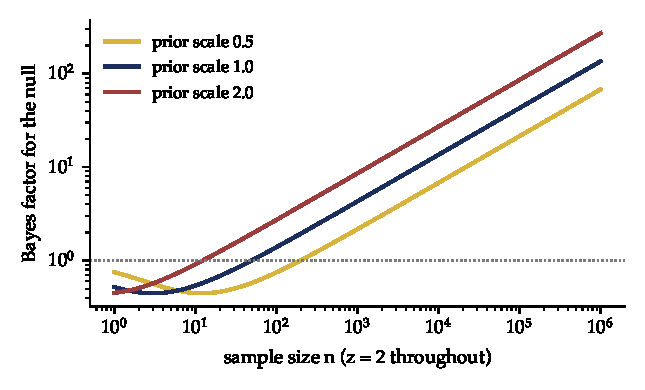
\includegraphics[width=\linewidth]{fig_lindley}
\caption{Lindley's paradox. With the $z$ statistic held at two, the Bayes factor in favour of the null hypothesis grows with the sample size, for each of three prior scales on the alternative.}
\label{fig:lindley}
\end{figure}

The paradox matters in litigation because modern cases often involve large data sets: millions of transactions in a price fixing case, every hiring decision of a national employer, all the trades in a market manipulation inquiry. In such cases trivial deviations from a null hypothesis become statistically significant. The question the court must answer is not whether the deviation is zero but whether it is large enough to matter, and whether the claimant's account predicts the data better than the defendant's. A Bayes factor comparing two substantively specified hypotheses, for instance a hiring rate equal to the qualified labour pool against a rate reduced by a meaningful margin, answers that question directly.

\section{Sensitivity and robustness}

The objection to Bayes factors most often heard in court is that they depend on priors for parameters, and so are subjective. The answer is that the dependence should be reported, not hidden. A forensic report or an expert's evidence should show the Bayes factor over a range of reasonable priors, and the conclusion should be stated in terms that hold across that range. If the Bayes factor exceeds one thousand for every prior an informed person could reasonably hold, the evidence is strong; if it ranges from two to two thousand, the report should say so, and the fact finder must weigh the expert's reasons for preferring one end.\index{robustness}

There is a formal theory of such ranges. Robust Bayesian analysis computes the infimum and supremum of the posterior or the Bayes factor over a class of priors, such as all priors within a given distance of a reference prior or all priors with specified quantiles \citep{berger1994}. For legal use the classes should be defined by what the parties can argue about: the population frequency of a feature, the error rate of a laboratory, the prior probability that a defendant had access to an item. The resulting interval of Bayes factors is a natural thing for an expert to report.

\begin{casebox}{A worked example: footwear marks}
A shoe print at a scene matches the defendant's shoe in pattern, size and two wear features. Suppose the pattern is shared by between one and five per cent of shoes in circulation, the size by about ten per cent of shoes of that pattern, and each wear feature by between five and twenty per cent of shoes of that pattern and size, independently. The Bayes factor lies between
\begin{gather*}
\frac{1}{0.05\times 0.1 \times 0.2 \times 0.2} = 5{,}000 \quad\text{and}\quad\\ \frac{1}{0.01\times 0.1\times 0.05\times 0.05} = 400{,}000 .
\end{gather*}
Even the lower bound is strong evidence that the shoe made the mark. In \emph{R v T} the expert gave a verbal conclusion that rested on an undisclosed likelihood ratio, computed from frequency data that the Court of Appeal found unreliable \citep{rvt2010}; Chapter~\ref{ch:odds} describes the case. Stating the inputs and their ranges answers the concern about transparency, while whether the footwear database can support any such figure remains a matter of argument \citep{berger2011}.
\end{casebox}

\section{Hierarchical models for forensic frequencies}

Many forensic frequencies are estimated from small databases. A glass fragment's refractive index, a fibre's dye, a toolmark's striations: each is compared with a reference collection of modest size. The uncertainty in the frequency is then substantial, and the Bayes factor should reflect it. If the observed count of a feature in a database of size $n$ is $k$, and the frequency $\gamma$ has a beta prior $\text{Beta}(a,b)$, the predictive probability that a new random item shares the feature is
\begin{equation}
\Prob(\text{match}\given k,n) = \frac{k + a}{n + a + b},
\label{eq:betapred}
\end{equation}
which for $k = 0$ gives $a/(n+a+b)$ rather than zero. This simple formula is the Bayesian answer to the frequent embarrassment of a feature never before seen in a database. With a uniform prior, $a = b = 1$, a feature unseen in a database of one hundred has predictive frequency about one per cent; once the suspect's own item is counted as a further observation the conditional match probability is $2/103$, and the Bayes factor is about fifty, not infinity.\index{hierarchical model}

When features come from several populations, a hierarchical model pools information across them while allowing each its own frequency. This is the structure of the subpopulation correction in DNA statistics, where the parameter $\theta$, often called $F_{ST}$, measures the excess relatedness within a subpopulation. The Balding and Nichols formula for the conditional match probability of a heterozygote,
\begin{equation}
\Prob(\text{match}) = \frac{2\,[\theta + (1-\theta)p_a][\theta + (1-\theta)p_b]}{(1+\theta)(1+2\theta)},
\end{equation}
is the predictive probability under a Dirichlet model for allele frequencies in the subpopulation \citep{balding2005}.

\section{Bayes factors for stories and theories}

The Bayes factor applies to any pair of hypotheses that make predictions, not just to forensic identification. In civil litigation the competing hypotheses are often whole theories of what happened: that a company knew of a defect and concealed it, or that it discovered the defect only later; that a trader manipulated a benchmark, or that his submissions reflected his honest view of the market. Each theory predicts the documents, emails and trading records, and the Bayes factor measures which theory predicts them better. Chapter~\ref{ch:stories} develops this idea as a theory of legal stories.

A useful way to think of a composite theory is as a mixture over subplots. The claimant's theory $\Hp$ is a set of possible histories, each with a prior weight; its marginal likelihood is the weighted average of the probability of the evidence under each history. A theory that fits the evidence only under a narrow set of improbable assumptions has a low marginal likelihood, because the assumptions carry little prior weight. This is the Bayesian form of Occam's razor, and it sits naturally with Lord Brandon's warning in \emph{The Popi M} that a judge is not bound to choose between two improbable explanations \citep{popim1985}. A court may conclude that neither party's account is probable enough to discharge the burden.

\section{Communicating Bayes factors}

Fienberg and Kadane, writing in 1983, set out principles for presenting Bayesian analyses in legal proceedings \citep{fienberg_kadane1983}. The analyst should state the model and the prior clearly, show the results under the priors that the opposing party is likely to favour, and avoid presenting a single posterior probability of guilt, which usurps the role of the fact finder. Over forty years later these principles remain sound. We would add three more. First, report the Bayes factor on the log scale as well as the natural scale, because people find additive weights easier to compare than multiplicative factors. Second, distinguish the source question, whose trace this is, from the activity question, how the trace got there, and report a Bayes factor only for the question it actually addresses. Third, give the fact finder a picture, such as Figure~\ref{fig:posterior} here and Figure~\ref{fig:population} of Chapter~\ref{ch:odds}, which show the posterior over a range of priors, so that the consequences of their own judgments are visible.

\begin{figure}[t]
\centering
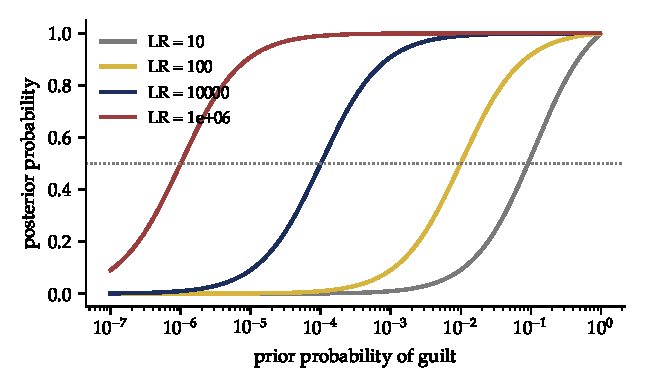
\includegraphics[width=\linewidth]{fig_posterior_odds}
\caption{Posterior probability as a function of the prior probability for four likelihood ratios. A Bayes factor of a million moves a prior of one in a hundred thousand to about $0.9$; a factor of one hundred leaves it close to zero.}
\label{fig:posterior}
\end{figure}

\section*{Notes and Questions}
\addcontentsline{toc}{section}{Notes and Questions}
\begin{enumerate}[label=\arabic*.]
\item Derive \eqref{eq:dnaerror} from a model in which a reported match occurs either because the profiles truly match or because of laboratory error. Under what conditions is the approximation poor?
\item Evaluate \eqref{eq:sbb} for $p = 0.05, 0.01, 0.001$. Compare these bounds with the posterior probabilities a court might mistakenly read off from the p values.
\item Using \eqref{eq:lindleybf} with $\tau = 1$, find the sample size at which a $z$ statistic of $2.5$ becomes evidence for the null.
\item A fibre type is absent from a database of $250$ garments. Using \eqref{eq:betapred}, with the suspect's own item counted as a further observation, and $a = b = 1$, compute the Bayes factor for a match. Repeat with $a = 0.5$, $b = 0.5$.
\item In the footwear casebox, suppose the two wear features are positively correlated, so that given the first the probability of the second doubles. Recompute the bounds.
\item Construct an example of two composite theories in a civil case, specify priors over their subplots, and compute the marginal likelihoods of a set of three documents. Explain how the Bayesian Occam factor appears.
\end{enumerate}

\section*{Further reading}
Kass and Raftery's review remains the best introduction to Bayes factors \citep{kass1995}. On robustness see Berger \citep{berger1994}. On DNA, Balding \citep{balding2005} and the NRC report \citep{nrc1996}. Thompson's work on laboratory error is essential reading \citep{thompson2003}.
